\chapter{Methodology}
\label{ch:method}

This chapter details the overarching system methodology, architectural principles, software lifecycle model, and pedagogical design underpinning \textbf{CodeQuest AI}. It describes the interaction loops between player actions, game-state transitions, network requests, asynchronous code execution, and persistent progress tracking.

\section{System Architecture and Paradigm}
CodeQuest AI is architected as an asynchronous, distributed client-server ecosystem designed to separate high-frequency game rendering from compute-intensive, secure code evaluation. Figure~\ref{fig:arch_flow} illustrates the four primary tiers comprising the platform:
\begin{enumerate}
    \item \textbf{Presentation \& Client Gameplay Tier (Unity 6 URP):} Executes locally on the student workstation, rendering 3D graphics at 60\,FPS, managing third-person physics and camera controllers, presenting the UI canvas, and capturing code input.
    \item \textbf{Application \& Gateway Tier (FastAPI):} Asynchronous REST API service handling player session state, curriculum definitions, quest events, and dispatching evaluation jobs.
    \item \textbf{Sandboxed Code Execution Tier (Docker Evaluator):} Stateless worker service executing submitted Python source code inside isolated, unprivileged container instances.
    \item \textbf{Data Persistence \& Identity Tier (PostgreSQL \& Keycloak):} Relational storage of immutable submission records and versioned progress snapshots, governed by OpenID Connect authorization tokens.
\end{enumerate}

\begin{figure}[htbp]
    \centering
    \begin{minipage}{0.9\textwidth}
        \centering
        \setlength{\fboxsep}{10pt}
        \setlength{\fboxrule}{0.8pt}
        \fbox{
        \begin{minipage}{0.95\textwidth}
            \centering
            \textbf{\large CodeQuest AI --- Tiered System Interaction}\\[0.4cm]
            \framebox[0.9\textwidth]{\textbf{Unity 6 3D Client} (Third-Person Controller $\leftrightarrow$ In-Game Code Editor)}\\[0.3cm]
            $\Downarrow$ \quad \textit{HTTP/JSON REST Requests (PKCE Bearer Token)} \quad $\Uparrow$\\[0.3cm]
            \framebox[0.9\textwidth]{\textbf{FastAPI Backend Gateway} (Curriculum Catalog $\leftrightarrow$ Quest State Machine)}\\[0.3cm]
            $\swarrow$ \hspace{4cm} $\searrow$\\[0.3cm]
            \framebox[0.42\textwidth]{\textbf{PostgreSQL 17 Datastore}\newline (Profiles, Quests, Submissions)} \hfill
            \framebox[0.45\textwidth]{\textbf{Docker Python Sandbox}\newline (Timeouts, Memory Limits, Test Runner)}\\[0.2cm]
        \end{minipage}
        }
    \end{minipage}
    \caption{High-Level Architectural Data Flow of CodeQuest AI}
    \label{fig:arch_flow}
\end{figure}

\section{Pedagogical Challenge and Curriculum Design}
The pedagogical curriculum in CodeQuest AI follows cognitive scaffolding and constructive alignment. Learning objectives are mapped directly onto thematic zones:
\begin{itemize}
    \item \textbf{Variable Valley (Zone 1):} Focuses on variable assignment, dynamic typing, primitive data types (integers, floats, strings, booleans), basic arithmetic, string interpolation (f-strings), and standard function input/output.
    \item \textbf{Condition Canyon (Zone 2, Planned):} Decision-making structures, relational operators, compound boolean logic, nested branching, and match-case statements.
    \item \textbf{Loop Lagoon (Zone 3, Planned):} Iteration paradigms, \texttt{for} sequences, \texttt{while} guards, loop control (\texttt{break}, \texttt{continue}), and range manipulations.
    \item \textbf{Function Forest (Zone 4, Planned):} Modular parameter passing, default arguments, keyword arguments, scope resolution, and recursion.
\end{itemize}

In the implemented vertical slice (Variable Valley), the curriculum interface displays an ordered sequence of challenges and concrete learning goals, as depicted in Figure~\ref{fig:learning_region_catalog}.

\begin{figure}[htbp]
    \centering
    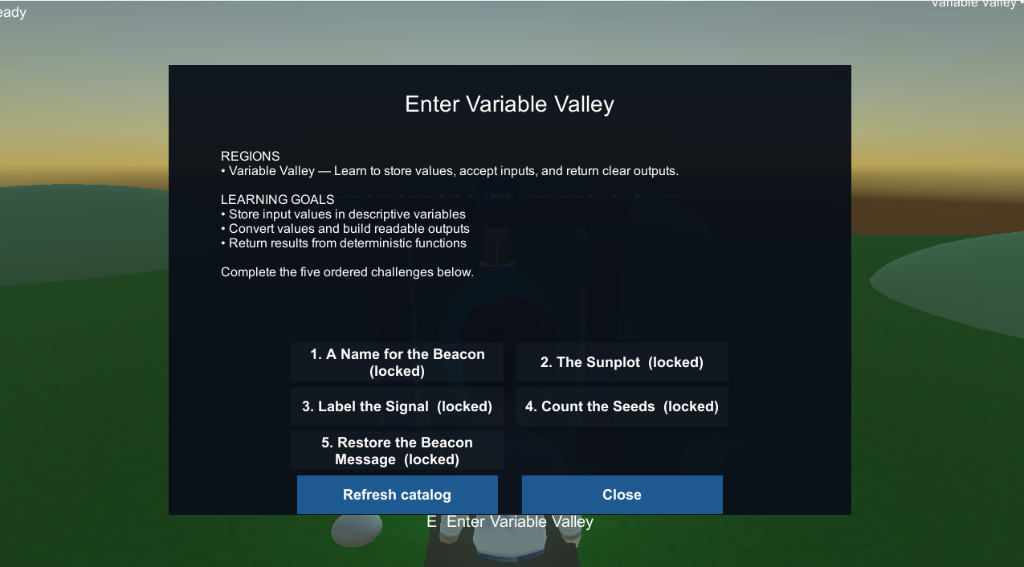
\includegraphics[width=0.84\textwidth]{figures/learning_region_catalog.png}
    \caption{Variable Valley Curriculum Catalog and Learning Region Interface}
    \label{fig:learning_region_catalog}
\end{figure}

Challenge 1 (\texttt{valley-name-tag}) requires the learner to implement a formatting function \texttt{make\_name\_tag(name)} returning a greeting string \texttt{"Hello, \{name\}!"}. The challenge enforces:
\begin{enumerate}
    \item Correct functional signature matching curriculum specifications.
    \item Handling arbitrary string inputs without hard-coding specific test literals.
    \item Satisfying both visible test cases (Ada, Kai) and hidden test suites (Grace) to prevent trivial test-case cheating.
\end{enumerate}

\section{Player Interaction and Challenge Activation Loop}
The player interaction loop is designed to minimize cognitive friction while maintaining immersive gameplay context:
\begin{enumerate}
    \item \textbf{Exploration \& Discovery:} The player moves through the 3D world using standard keyboard controls (WASD, Space for jumping, Shift for sprinting). Proximity detection triggers an interaction prompt on the HUD (\texttt{"E Inspect Valley Beacon"}).
    \item \textbf{Contextual Engagement:} Pressing \texttt{E} activates the \texttt{ChallengeBeaconInteractable} component, which pauses player movement, unlocks the mouse cursor, and transitions the game state from \texttt{InWorld} to \texttt{ChallengeModal}.
    \item \textbf{Code Composition:} The learner types Python code directly into the multiline editor. The editor features monospace typography (Consolas TrueType), tab indentation support, and clipboard shortcuts.
    \item \textbf{Execution Trigger:} Clicking \texttt{"$\blacktriangleright$ Run / Submit"} packages the editor text into a submission payload and initiates the asynchronous evaluation pipeline.
\end{enumerate}

\section{Asynchronous Code Execution and Sandboxing Protocol}
To maintain responsiveness and protect infrastructure security, code execution is processed asynchronously through a strict multi-stage pipeline:
\begin{enumerate}
    \item \textbf{Client Dispatch:} The Unity client generates a cryptographically random submission UUID and dispatches a \texttt{POST /api/v1/challenges/\{slug\}/submissions} request containing the source code and an idempotency token.
    \item \textbf{Backend Ingestion:} The FastAPI gateway validates that the challenge slug and version are active, records an initial \texttt{pending} submission record in PostgreSQL, and enqueues the evaluation job.
    \item \textbf{Sandbox Execution:} The evaluator worker mounts the source code into an ephemeral Python container (\texttt{codequest-evaluator:local}) with:
    \begin{itemize}
        \item Execution timeout enforced at 5,000\,ms via OS signal alarms.
        \item Memory consumption capped at 128\,MB with no network access enabled.
        \item Standard output and error buffers intercepted and capped at 64\,KB.
    \end{itemize}
    \item \textbf{Test Suite Execution:} The test harness executes unit assertions against the submitted code, capturing assertion failures, syntax errors, and tracebacks.
    \item \textbf{Result Streaming \& HUD Feedback:} The backend retrieves the structured result and returns it upon the client's next poll. The Unity client updates the output card with emerald green indicators for passed test cases or specific error feedback for failed runs.
\end{enumerate}

\section{Progress Persistence and Idempotency}
To prevent network disruptions or accidental double-submissions from corrupting student records, quest progression relies on server-authoritative state transitions. Every event (e.g., interacting with Mira, completing a checkpoint, or passing an evaluator test) produces a unique client event ID. The backend verifies event sequences against quest objective prerequisite graphs before updating the persistent snapshot, ensuring full data consistency across client restarts.
